\chapter{Specific Requirements}

\section{Functional Requirements}
% \subsection{Stimulus/Response Sequences}
% $<$List the sequences of user actions and system responses that stimulate the
% behavior defined for this feature. These will correspond to the dialog elements
% associated with use cases.$>$
\begin{flushleft}
\begin{itemize}
	\item  [\textbf{R1:}] FMDS will \textbf{follow} the ranger

		\begin{itemize}
			\item  [\textbf{R1.1}] FMDS will allow the ranger to perform \textbf{initialisation} for the drone.
				\begin{itemize}
					\item [\textbf{R1.1.1}] FMDS will allow the ranger to set himself as the validated object.
					\item [\textbf{R1.1.2}] FMDS will allow the ranger to initialise his beacon. 
				\end{itemize}

			\item  [\textbf{R1.2}] FMDS will allow the ranger to specify a \textbf{flight pattern} for the drone
				\begin{itemize}
					\item [\textbf{R1.2.1}] FMDS will detect objects while on its flight path.
					\item [\textbf{R1.2.2}] FMDS will record while on its flight path.
				\end{itemize}

			\item  [\textbf{R1.3}] FMDS will receive \textbf{location updates} from the rangers beacon.
				\begin{itemize}
					\item  [\textbf{R1.3.1}] FMDS will move itself to the new location during its patrol
				\end{itemize}
		\end{itemize}
\end{itemize}

\begin{itemize}
	\item [\textbf{R2:}] FMDS will \textbf{patrol} the area around the ranger

		\begin{itemize}
			\item [\textbf{R2.1}] FMDS will patrol by flying in the designated \textbf{flight pattern} around the ranger.
			\item [\textbf{R2.2}] FMDS will perform \textbf{object detection}.
				\begin{itemize}
					\item [\textbf{R2.2.1}] FMDS will drop a pin of the object detected on the 2D map.
				\end{itemize}
			\item [\textbf{R2.3}] FMDS will \textbf{record} during it's surveillance.
			\item [\textbf{R2.4}] FMDS will take \textbf{snapshots} of the reserve during it's surveillance.
				\begin{itemize}
					\item [\textbf{R2.4.1}] FMDS will build a 2D map of the reserve.
				\end{itemize}
		\end{itemize}
\end{itemize}

\begin{itemize}
	\item  [\textbf{R3:}] FMDS will \textbf{detect objects} in the reserve

		\begin{itemize}
			\item  [\textbf{R3.1}] FMDS will allow the ranger to see a list of \textbf{objects} and their \textbf{locations}.
		\end{itemize}
\end{itemize}

\begin{itemize}
	\item  [\textbf{R4:}] FMDS will build a \textbf{2D map} of the reserve

		\begin{itemize}
			\item  [\textbf{R4.1}] FMDS will use the snapshots taken to build a 2D map of where it has flown.
		\end{itemize}
\end{itemize}
\end{flushleft}


\section{Use Case Diagram}

	\begin{figure}[h!]
		\centering
		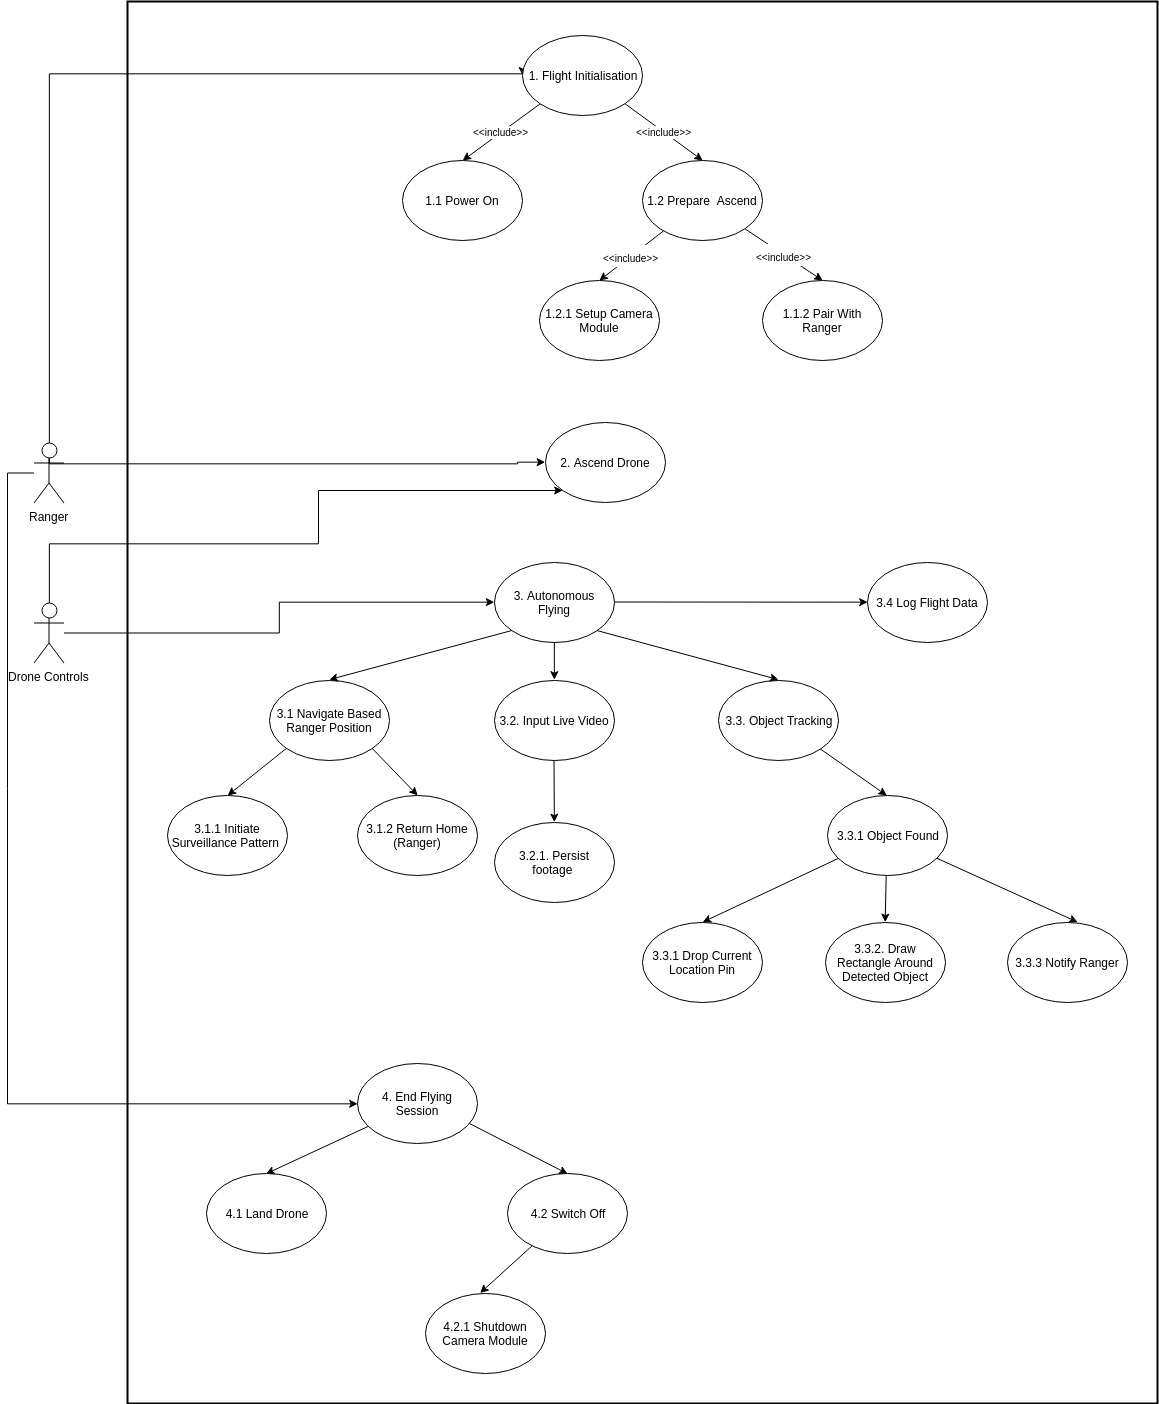
\includegraphics[scale=0.35]{./assets/images/uc-diagram-1.jpg}
		\label{fig: use-case-diagram}
		\caption{Use Case Diagram}
	\end{figure}



